\begin{figure}[t!]
    \centering
    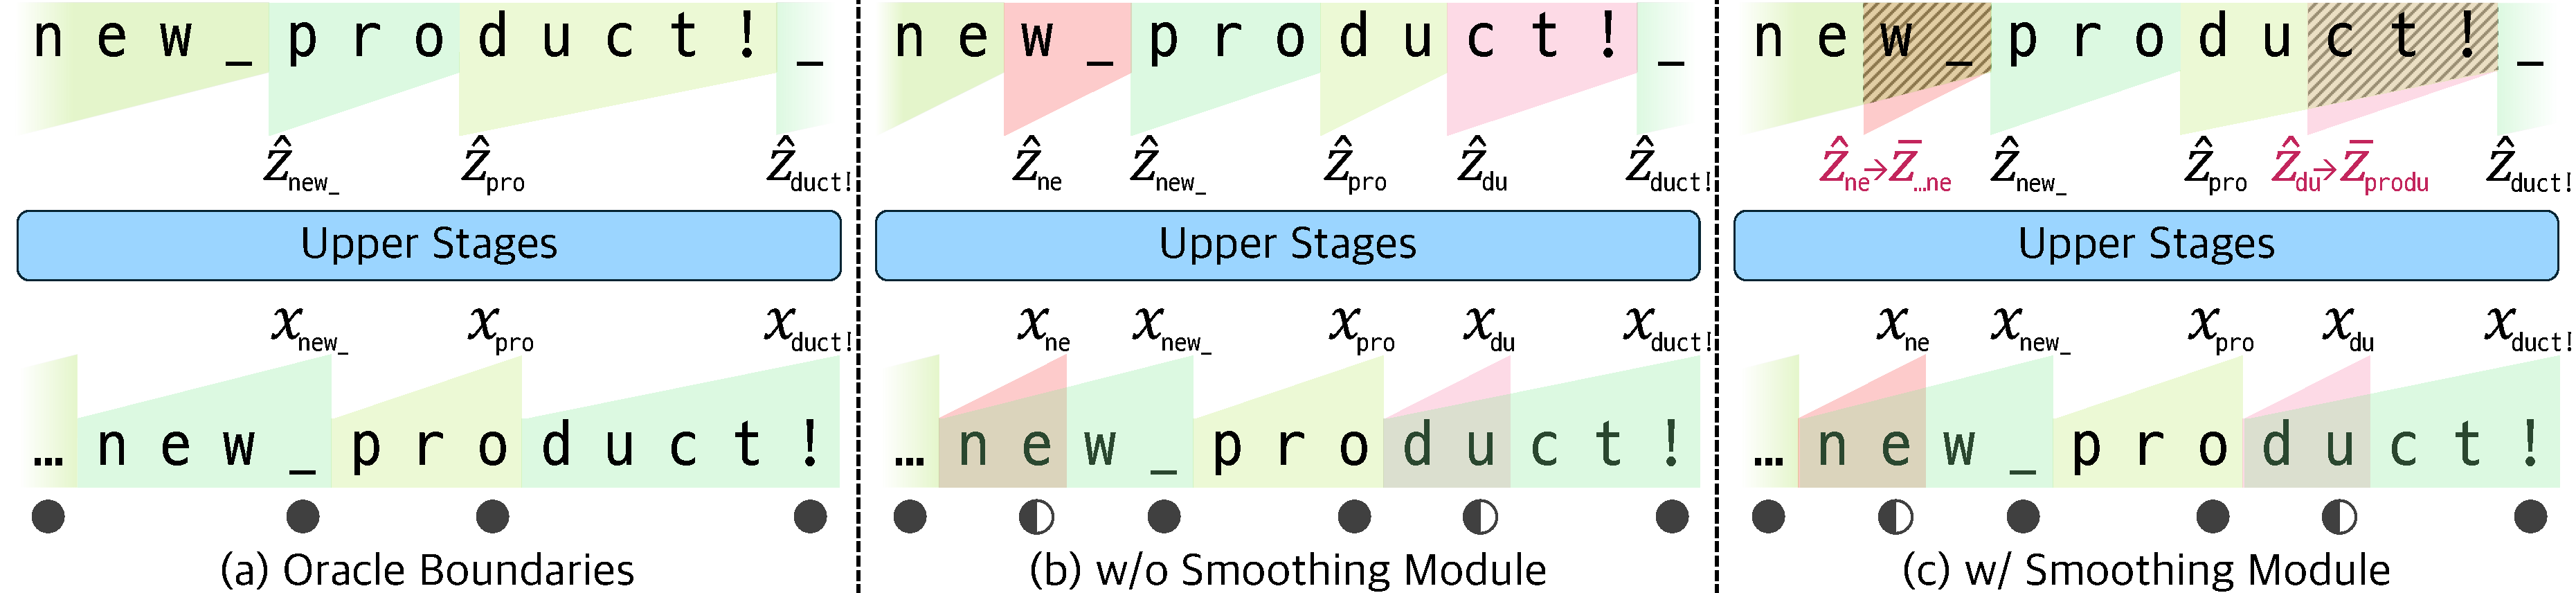
\includegraphics[width=1.0\linewidth]{fig_img/new_product.pdf}
    \caption{
    Comparison of decompression strategies on the example sequence \texttt{"...new product!"}.
    $\CIRCLE$ indicates a boundary with high confidence ($P_t=1.0$) and $\LEFTcircle$ indicates a boundary with low confidence ($P_t=0.5$).
    As each letter in the example is unique, we use the letters in subscripts to denote expected semantics of chunks.
    (a) Optimal chunking with oracle boundaries identifying linguistically meaningful units.
    (b) Suboptimal chunking without a \smoother{}.
    This creates misalignment during upsampling, causing information from incorrect contexts to propagate.
    (c) Improved decompression with a \smoother{}, where low-confidence chunks are interpolated with weighted combinations of previous chunks, correcting the shaded regions.
    In panels (b) and (c), we interpret low-confidence boundaries cause the encoder network to embed broader contexts at subsequent positions.
    Specifically, the vectors at \texttt{\_} and \texttt{!} encode \texttt{new\_} and \texttt{duct!}, respectively (instead of \texttt{w\_} and \texttt{ct!}).
    }
    \label{fig: new_product}
\end{figure}
